\documentclass[prb,aps,nobibnotes,twocolumn,doublespace,twocolumngrid,superbib]{revtex4}
%\documentclass[prb,aps,nobibnotes,superbib,preprint]{revtex4}

\usepackage{graphicx}
\usepackage{amsfonts}
\usepackage{amsmath}
\usepackage{bm}
\usepackage{alltt}
\usepackage{dcolumn} 
\usepackage{graphicx}
\makeatletter 
\makeatother

\begin{document}

\title{\textbf{Linear scaling computation of the Fock matix VIII. The exchange matrix
for periodic systems}}


\author{C. J. Tymczak}
\author{Matt Challacombe}

\affiliation{Theoretical Division, Los Alamos National Laboratory, Los Alamos,
New Mexico 87545 }

\date{\today}

\begin{abstract}
We report on a consistent derivation of the exchange matrix for periodic
systems at the Gamma point. Previous work has always included k-space integration 
within the calculation of the exchange matrix. However, in  these methods
we can show that the calcaulation of the exchange matrix becomes inconsistent as the
region of k-space shrinks. This leads to a non-translationally invarient exchange matrix,
which is of major concern. We illustrate this problem and then show how, by a set of
simple ideas and arguments, we can correct this problem.
\end{abstract}

\maketitle

\section{Introduction}



\section{The Hartree Fock Equations}


\subsection{The Exchange matrix}



\section{Verification}

\subsubsection{Magnesium Oxide}

Table \ref{table:ComToCrystal98_2} shows our results for the total
energy for Magnesium Oxide as compared to results obtained from \textbf{Crystal98}.
Because of the high degree of Ionic bounding in this system, \textbf{Crystal98}
does substantially better then for sodium Chloride. This allows for
a much closer scrutiny of the energies then for the previous system.
Again, we obtain excellent agreement with \textbf{Crystal98} for two
different basis sets and theory levels to within the accuracy of these
results.Also,in Table \ref{table:ComToCrystal98_2}
we show the convergence of the energy per atom of a Magnesium Oxide
test system for increasing system size and we also has excellent agreement
with \textbf{Crystal98} results in which we do k-space integration.



\section{Scaling}

For testing of linear scaling, we us a set of periodic diamond systems.
Figure \ref{figure:Scaling_Matrix_Build} shows our scaling results
of diamond periodic system for both the \( J_{QCTC} \) and \( K_{xc} \)
matrix builds for the \textbf{Crystal98} basis set 6-21G* \cite{C98Basis}
at a {\it good} accuracy. Even in this very dense periodic system for a medium 
basis set with d-functions, linear scaling for the matrix build commences very 
early. We also show in figure \ref{figure:EnergyPerN} the energy per carbon atom and 
in figure \ref{figure:ErrorPerN} the relative error in the total energy. 
Again we see the convergence of the total energy
as a function of increasing system size, which is akin to k-space integration. We also
see that our relative error is very well controlled within the \textbf{MondoSCF} quantum
chemistry code, even up to 512 carbon atoms.


\section{CONCLUSIONS}


\section*{ACKNOWLEDGMENTS}

We would like to acknowledge Tommy Sewell and Ed Kober for there advise
and support. We would also like to thank Anders Niklasson for his help
in preparation of this manuscript. 

\bibliographystyle{apsrmp} 
\bibliography{mondo}


\eject

\begin{table}
\caption{Comparison \textbf{MondoSCF} and \textbf{Crystal98} for a 
Sodium Chloride test system. The \textbf{MondoSCF} calculations where done to
the accuracy of the quoted digits. All calculations where done at the Gamma point
for comparison except the last \textbf{Crystal98} calculation, which was done at ${\bf k}=(6,6,6)$.
The \textbf{Crystal98} 8-511G  basis set was used \cite{C98Basis} and the BLYP gradient corrected 
functional \cite{Becke93}.}
\label{table:ComToCrystal98_1}
 
\begin{tabular}{clcll}
\hline 
Prog&
Basis/Theory&
\( N \)&
Energy  (au)&
Energy/{\it N}\\
\hline
\hline 
M &
STO-3G/HF &
2 &
-270.79309374 &
-135.39654687 \\
M&
STO-3G/HF&
8&
0.0 &
0.0 \\
M&
STO-3G/HF&
64&
-8678.94684605 &
 -135.60854447 \\
\hline
C&
STO-3G/HF&
2&
-271.21819 &
-135.60910 \\
\hline 
\hline
\end{tabular}
\end{table}

\begin{figure}
\caption{Simulation cell and its brava lattice vectors.}
\label{figure:SimCell}
{\centering \includegraphics{UnitCell_2.ps} \par}
\end{figure}
%
%
%
\begin{figure}
\caption{The region in which atom $a$ has exchange interactions}
\label{figure:ExchangeRegion}
{\centering \includegraphics{ExchangeRegion.ps} \par}
\end{figure}
%
%
%
\begin{figure}

\caption{\label{figure:Scaling_Matrix_Build} Scaling Results for the matrix
builds \protect\( J_{QCTC}\protect \) and \protect\( K_{xc}\protect \)
for the dense diamond periodic system up to 512 atoms using the
{\bf Crystal98} basis set 6-21G* \cite{C98Basis} and the density functional BLYP \cite{Becke93}}

{\centering \includegraphics{UnitCell_2.ps} \par} 
\end{figure}
%
%
%
\begin{figure}

\caption{\label{figure:EnergyPerN} Energy per carbon atom for the dense diamond
periodic system up to 512 atoms using the {\bf Crystal98} basis set 6-21G* \cite{C98Basis} and the 
density functional BLYP \cite{Becke93}}

{\centering \includegraphics{UnitCell_2.ps} \par} 
\end{figure}
%
%
%
\begin{figure}

\caption{\label{figure:ErrorPerN} Relative Error per carbon atom for the dense diamond
periodic system up to 512 atoms using the {\bf Crystal98} basis set 6-21G* \cite{C98Basis} and the 
density functional BLYP \cite{Becke93}}

{\centering \includegraphics{UnitCell_2.ps} \par} 
\end{figure}



\end{document}
